\documentclass{article}
\usepackage{hyperref}
\usepackage{amsmath}
\usepackage{amsfonts}
\usepackage{graphicx}\graphicspath{{figs}{.}}
%\usepackage[margin=1in]{geometry}

\title{Denoising in Electron Microscopy Imaging}

\author{Vicente González-Ruiz and José Jesús Fernández Rodríguez}

\begin{document}
\maketitle

\begin{abstract}
  We analyze the denoising performance of signal averaging for several
  noise statistical distributions. Then, we perform an objective
  comparison between some of the denoising algoritms in the field
  of 3D Electron Microscopy, in two situations, when we have a
  denoised version of the signal and we have not.
\end{abstract}

\section{Metrics}

The following metrics have been used to compare the noisy (original)
volume and the denoised volume.

\subsection{\href{https://en.wikipedia.org/wiki/Mean_squared_error}{MSE (Mean
    Squared Error)}}

Having two volumes $\mathbf{X}$ and $\mathbf{Y}$,
\begin{equation}
  \text{MSE}(\mathbf{X},\mathbf{Y}) = \frac{1}{N}\sum_{i=1}^N(\mathbf{X}_i - \mathbf{Y}_i)^2,
\end{equation}
where $N$ is the number of samples in one of the volumes (that must
have the same number of samples).

\subsection{\href{https://en.wikipedia.org/wiki/Structural_similarity_index_measure}{SSIM
    (Structural Similarity Index Measure)}}

After splitting the volume into $M$ non overlapped sub-vols,
\begin{equation}
  \text{SSIM}(\mathbf{X}, \mathbf{Y}) := \frac{1}{N} \sum_{i=1}^N \frac{(2\overline{\mathbf{x}}_i \overline{\mathbf{y}}_i + c_1)(2\sigma_{\mathbf{x}_i \mathbf{y}_i} + c_2)}{(\overline{\mathbf{x}_i^2} + \overline{\mathbf{y}_i^2} + c_1)(\sigma^2_{\mathbf{x}_i} + \sigma^2_{\mathbf{y}_i} + c_2)},
\end{equation}
where $\overline{x}i$ is the mean of the $i$-th sub-vol of
$\mathbf{X}$, $\sigma^2_{\mathbf{x}_i}$ is its variance (equivalently
for $\mathbf{Y}$), $\sigma_{\mathbf{x}_i\mathbf{y}_i}$ is the
covariance of both sub-vols, $c_1=(k_1L) ²$, $c_2=(k_2L) 2$ are two
variables to stabilize the division with weak denominator, $L$ is the
dynamic range of the voxel values, with constants with default vales
$K_1=0.01$ , and $k_2=0.03$, and where the default size of the local
sub-vols is $7\times 7\times 7$.

\subsection{\href{https://en.wikipedia.org/wiki/Pearson_correlation_coefficient}{PPC
    (Pearson Correlation Coefficient)}}
The PPC is given by
\begin{equation}
  \text{PPC}(\mathbf{X}, \mathbf{Y}) := \frac{\sum_i(\mathbf{X}_i - \overline{\mathbf{X}})(\mathbf{Y}_i - \overline{\mathbf{Y}})}{\sqrt{\sum_i (\mathbf{X}_i - \overline{\mathbf{X}})^2 \sum_i (\mathbf{Y}_i - \overline{\mathbf{Y}})^2}}
\end{equation}

\subsection{FSC (Fourier Shell Correlation) curve}

Finally, notice that $\sigma$ (GD) is not (objectively) optimizable using
only pure distortion metrics, such as MSE, PCC, and SSIM.

The FSC curve is a measure of the similarity between two 3D volumes
represented in the Fourier domain \cite{verbeke2024self}. Each point
of the curve prepresents the correlation between two ``shells'' of
Fourier coefficients of both volumes. An advantage of the FSC over
other similarity metrics such as the MSE, the SSIM and the PPC is that
FSC values depend on the frequency, and this can be interesting in
some scenarios, such as microscopy, where the resolution of the
microscope is finite and known.

A FSC value of the FSC curve is determined by~\cite{verbeke2024self}
\begin{equation}
\text{FSC}(\mathbf{X}, \mathbf{Y}; r) := \frac{\sum_{i \in S_r} (\mathcal{F}(\mathbf{X)}_i \mathcal{F}(\mathbf{Y)}_i^*)}{\sqrt{\sum_{i \in S_r} |\mathcal{F}(\mathbf{X})_i|^2 \sum_{i \in S_r} |\mathcal{F}(\mathbf{Y})_i|^2}},
\end{equation}
where $i=(x, y, z)$ is a point (a coefficient in the Fourier domain)
of the surface of the sphere $S_r$ defined by $x^2+y^2+z^2=r^2$,
$\mathcal{F}(\cdot)$ is the Fourier transform of $\cdot$, and
$\cdot^*$ denotes the complex conjugate of $\cdot$.

In some fields such ashsingle particle electron cryo-microscopy
(cryo-EM), the FSC curve has become the universal resolution metric
and is used to assess the quality of a 3-D reconstruction
\cite{rosenthal2003optimal,scheres2012prevention}.

It is possible to compute the Self FSC (SFSC) by subsampling the data
\cite{koho2019fourier}, for example, splitting the volume in odd and
even slices, in each dimension (resulting a total of 6 subvolumes),
computing the FSC and averaging the correlations
\cite{verbeke2024self}. Another approach can split the data into two
random half volumes \cite{verbeke2024self}.

\section{Noise reduction by stacking noisy instances}
Let $\mathbf{X}$ be a \emph{clean} (without noise, ground truth
usually unknown) tensor\footnote{Which usually represents an image or
  a volume.}, and $\hat{\mathbf X}^{(i)}$ the $i$-th noisy-version
tensor random instance of $\mathbf{X}$ generated, in general, through
\begin{equation}
  \hat{\mathbf X}^{(i)} = f(\mathbf{X}, \mathbf{N}^{(i)}),
  \label{eq:general_model}
\end{equation}
where ${\mathbf N}^{(i)}$ the $i$-th (unknown) noise tensor instance
with the same shape as $\mathbf{X}$.

We assume that ${\mathbf X}$ and $\mathbf{N}$ are statistically
independent, and therefore, nothing can be said about
${\mathbf N}^{(i)}$ if we know $\hat{\mathbf X}^{(i)}$, and
viceversa, and therefore, it is impossible to obtain ${\mathbf X}$
from a single $\hat{\mathbf X}^{(i)}$, althouth we can approximate ${\mathbf X}$ by
averaging $\hat{\mathbf X}^{(i)}$ instances, performing
\begin{equation}
  \lim_{I \to \infty} \mathbb{E}\left[\{\hat{\mathbf X}^{(i)}\}_{i=1}^I\right] = \lim_{I \to \infty} \frac{1}{I} \sum_{i=1}^I \hat{\mathbf X}^{(i)} = {\mathbf X}.
  \label{eq:averaging_result}
\end{equation}
Notice that Eq.~\ref{eq:averaging_result} is true if 
\begin{equation}
  \overline{\mathbf N} = \lim_{I \to \infty}{\mathbb E}[\{{\mathbf N^{(i)}}\}_{i=1}^I]=\lim_{I \to \infty}\frac{1}{I} \sum_{i=1}^I {\mathbf N}^{(i)}={\mathbf 0},
  \label{eq:noise_expectation_2}
\end{equation}
where ${\mathbf 0}$ is the zero tensor with the same shape as
$\mathbf{X}$, and when $\overline{\mathbf N}\ne {\mathbf 0}$, but
known, we can still find ${\mathbf X}$ through
\begin{equation}
  {\mathbf X} = \lim_{I \to \infty} \mathbb{E}\left[\{\hat{\mathbf X}^{(i)}\}_{i=1}^I\right]  - \overline{\mathbf N},
  \label{eq:averaging_result_with_bias}
\end{equation}
where, in general, $\overline{\mathbf N}$ can be a function of the
amplitude of the noise.

As can be seen in Eq.~\ref{eq:averaging_result}, notice that we are
supposing an impossible scenario in which we have an infinite number
of noisy instances of the clean signal. Logically, in practice, $I$
will be finite and we will be able only to obtain an approximation of
${\mathbf X}$, that we denote by $\tilde{\mathbf X}$.

\section{Noise models}
\label{sec:noise_models}

\subsection{Signal-independent noise (SIN) models}
In SIN models, the noise is statistically i.i.d. (independent and
identically distributed), i.e., the random values of ${\mathbf N}^{(i)}$ satisfy that
\begin{equation}
  {\mathbb E}[\{{\mathbf N}^{(i)}_j\}_{j=1}^J]=\frac{1}{J} \sum_{i=1}^J {\mathbf N}_j^{(i)}=\overline{\mathbf N}^{(i)},
  \label{eq:noise_expectation_1}
\end{equation}
where ${\mathbf N}^{(i)}_j$ is the $j$-th (scalar) value
of ${\mathbf N}^{(i)}$, and
\begin{equation}
  J=\prod_{k=1}^D \mathbf{X}.\text{shape}[k],
\end{equation}
being $D$ the number of dimensions of the signal (in microscopy, usually 2 or 3).

SIN models, also called additive noise models, are defined by
\begin{equation}
  \hat{\mathbf X}^{(i)} = {\mathbf X} + {\mathbf N}^{(i)}.
  \label{eq:additive_noisy_model}
\end{equation}

Some examples of SIN are:
\begin{enumerate}
\item \textbf{Quantization noise}, that is usually modeled as additive
  zero-mean uniform noise (${\mathbf N}\sim{\mathcal U}(c)$) with PDF
  (Probability Density Function) defined as
  \begin{equation}
    f(x; c) = \Pr({\mathbf N}^{(i)}_j{=}x) = \begin{cases}
      \frac{1}{2c} & \text{for } -c \le x \le c, \\[8pt]
      0 & \text{for } x < c \ \text{ or } \ x > -c,
    \end{cases}
  \end{equation}
  $x$ and $f$ continuous, where $\Pr(\cdot)$ represents the
  probability of $\cdot$, and $c$ controls the amplitude of the
  noise. Notice that in this case, $\overline{\mathbf{N}}^{(i)}=0$ and
  therefore, $\overline{\mathbf N}={\mathbf 0}$ (see
  Eq.~\ref{eq:noise_expectation_2}). Fig.~\ref{fig:0MAUN} shows an
  example of how zero-mean uniform noise is cancelled by stacking.
  
  \begin{figure}
    \centering
    \resizebox{1.0\textwidth}{!}{
      \renewcommand{\arraystretch}{0.0} % Adjust row spacing in the table
      \setlength{\tabcolsep}{0ex}      % Adjust column spacing in the table    
      \begin{tabular}{cc}
        \href{https://nbviewer.org/github/vicente-gonzalez-ruiz/denoising/blob/main/figs/averaging_denoising.ipynb\#Display-Barb}{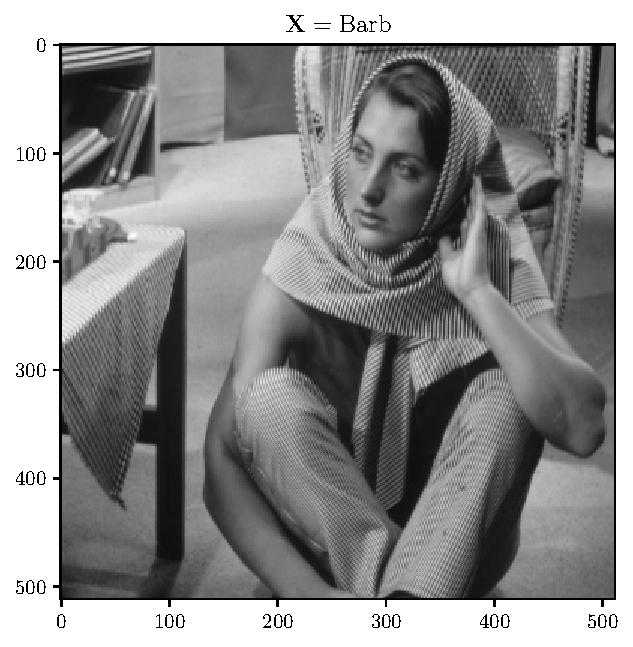
\includegraphics{barb}} & \href{https://nbviewer.org/github/vicente-gonzalez-ruiz/denoising/blob/main/figs/averaging_denoising.ipynb\#0MAUN_barb}{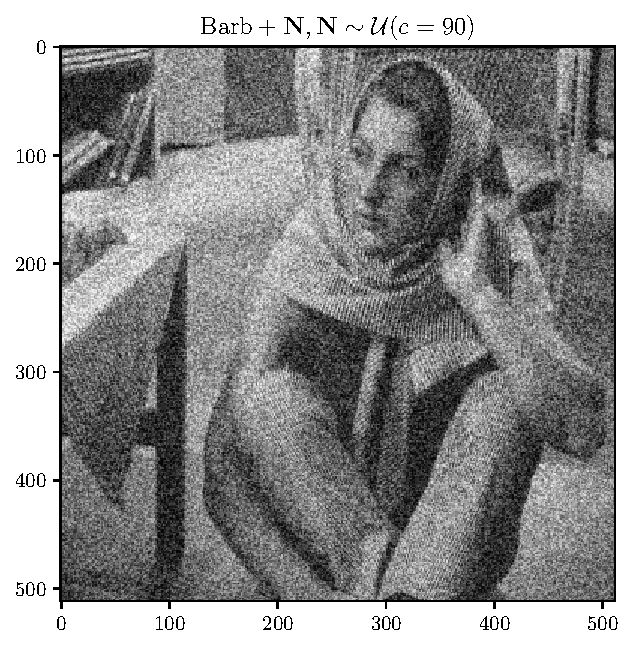
\includegraphics{0MAUN_barb}} \\
        \href{https://nbviewer.org/github/vicente-gonzalez-ruiz/denoising/blob/main/figs/averaging_denoising.ipynb\#denoised_0MAUN_barb}{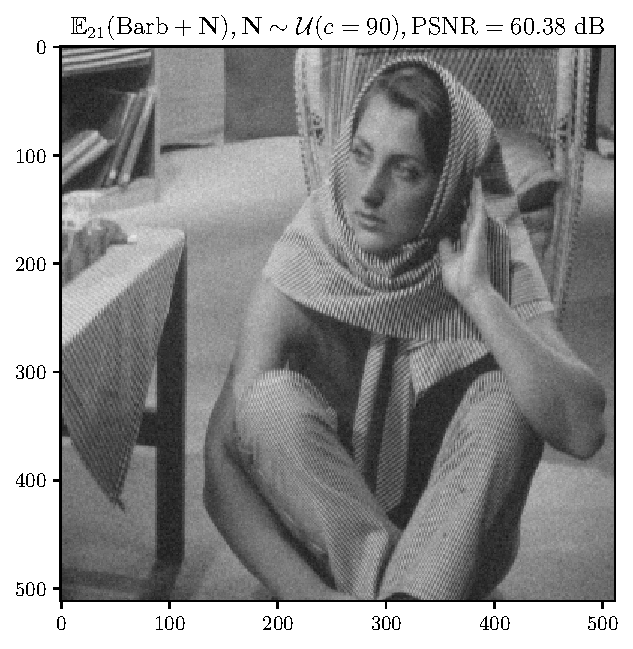
\includegraphics{denoised_0MAUN_barb}} & \href{https://nbviewer.org/github/vicente-gonzalez-ruiz/denoising/blob/main/figs/averaging_denoising.ipynb\#PSNR_0MAUN_barb}{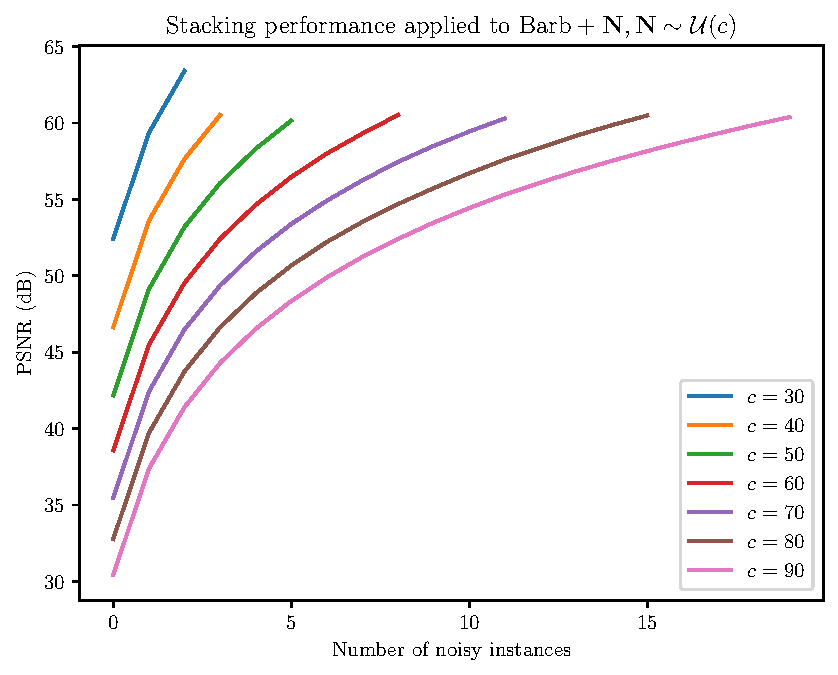
\includegraphics{PSNR_0MAUN_barb}}
      \end{tabular}
    }
    \caption{Effect of zero-mean additive uniform noise in an image
      and how stacking can be used to reduced by stacking. The clean
      image of Barb is shown on the top left, and a noisy version on
      the top right. On to bottom, the left image shows a denoised
      version after stacking and the right graph shows the performance
      of the stacking process for different levels of
      noise.\label{fig:0MAUN}}
  \end{figure}

\item \textbf{Thermal noise}, generally modeled as additive zero-mean
  Gaussian noise (${\mathbf N}\sim{\mathcal N}(\mu=0,\sigma^2)$, with
  PDF defined by
  \begin{equation}
    f(x; \sigma) = \Pr({\mathbf N}^{(i)}_j{=}x) = \frac 1 {\sigma\sqrt{2\pi}} e^{-\frac{x^2}{2\sigma^2} },
  \end{equation}
  $x$ and $f$ continuous, representing $\mu$ the mean and $\sigma$ the
  variance of the noise. Again, $\overline{\mathbf{N}}^{(i)}=0$ i.e.,
  $\overline{\mathbf N}={\mathbf 0}$. Fig.~\ref{fig:0MAGN} shows an
  example of how zero-mean Gaussian noise is cancelled by stacking.

  \begin{figure}
    \centering
    \resizebox{1.0\textwidth}{!}{
      \renewcommand{\arraystretch}{0.0} % Adjust row spacing in the table
      \setlength{\tabcolsep}{0ex}      % Adjust column spacing in the table    
      \begin{tabular}{cc}
        \href{https://nbviewer.org/github/vicente-gonzalez-ruiz/denoising/blob/main/figs/averaging_denoising.ipynb\#barb}{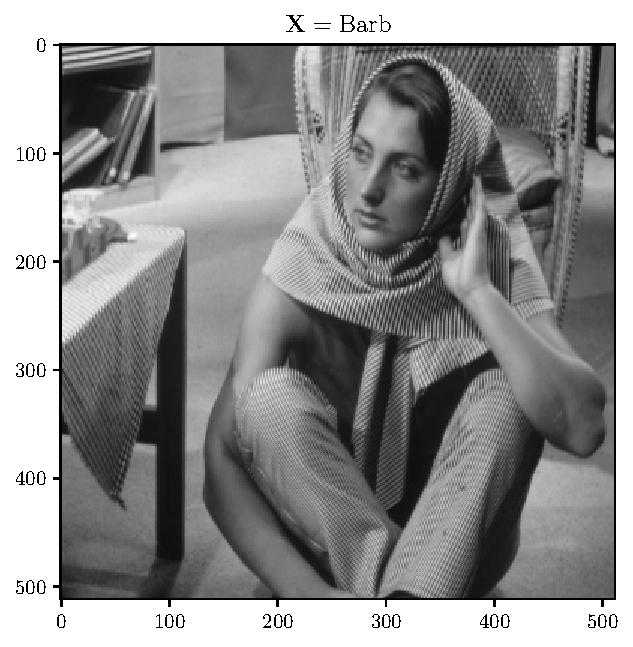
\includegraphics{barb}} & \href{https://nbviewer.org/github/vicente-gonzalez-ruiz/denoising/blob/main/figs/averaging_denoising.ipynb\#0MAGN_barb}{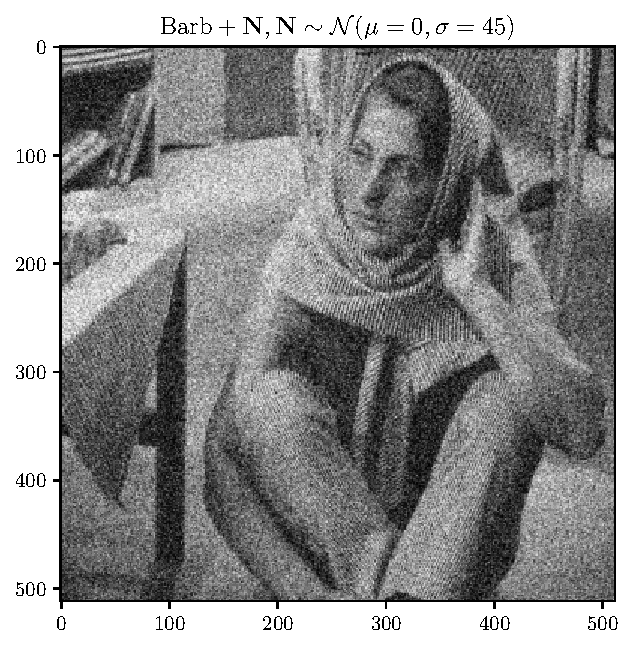
\includegraphics{0MAGN_barb}} \\
        \href{https://nbviewer.org/github/vicente-gonzalez-ruiz/denoising/blob/main/figs/averaging_denoising.ipynb\#denoised_0MAGN_barb}{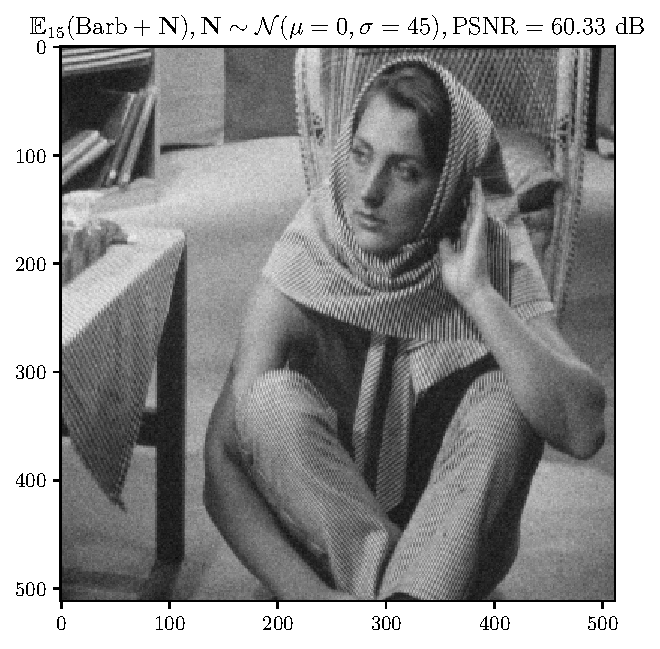
\includegraphics{denoised_0MAGN_barb}} & \href{https://nbviewer.org/github/vicente-gonzalez-ruiz/denoising/blob/main/figs/averaging_denoising.ipynb\#PSNR_0MAGN_barb}{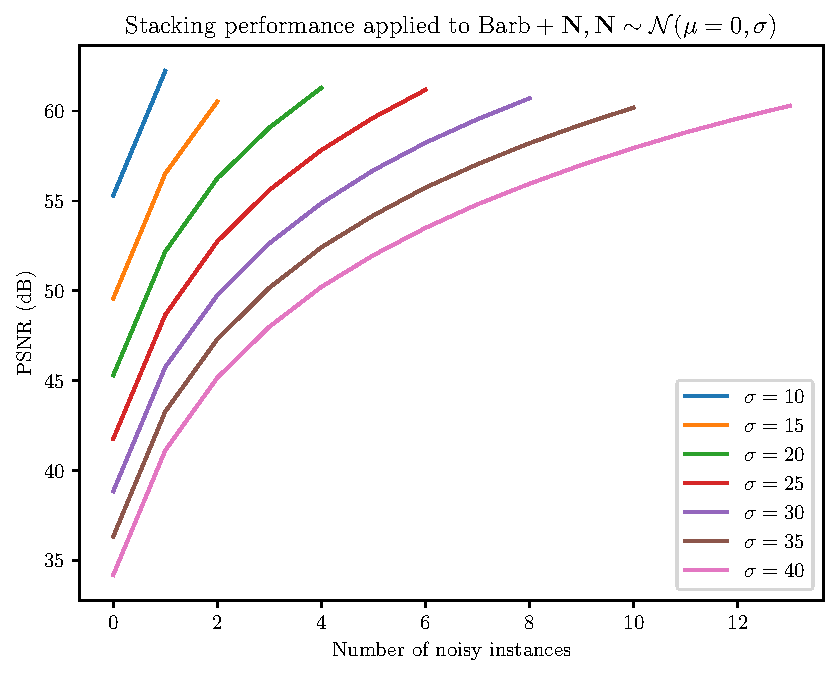
\includegraphics{PSNR_0MAGN_barb}}
      \end{tabular}
    }
    \caption{Effect of zero-mean additive Gaussian noise in an image
      and how stacking can be used to reduced by stacking. The clean
      image of Barb is shown on the top left, and a noisy version on
      the top right. On to bottom, the left image shows a denoised
      version after stacking and the right graph shows the performance
      of the stacking process for different levels of
      noise.\label{fig:0MAGN}}
  \end{figure}

\end{enumerate}

\subsection{Signal-dependent noise (SDN) models}
In SDN models, the amplitude of the random noise samples depends on
the clean signal (see Eq.~\ref{eq:general_model}).

%\begin{equation}
%  \hat{\mathbf X}^{(i)} = \mathbf{X} + {\mathbf N}^{(i)}(\mathbf{X}),
%  \label{eq:SDN_model}
%\end{equation}

Some SDN cases are:
\begin{enumerate}
\item \textbf{Speckle noise}, which can be considered multiplicative
  zero-mean Gaussian noise, modeled as
  \begin{equation}
    \hat{\mathbf X}^{(i)} = {\mathbf X} (1 + {\mathbf N}^{(i)}),
    \label{eq:MGN}
  \end{equation}
  where ${\mathbf N}\sim{\mathcal N}(\mu,\sigma)$. The noise present
  in synthetic aperture radar (SAR) and ultrasound images is usually
  considered speckle noise. Fig.~\ref{fig:0MMGN} shows an example of
  how zero-mean Gaussian noise is cancelled by stacking.

  \begin{figure}
    \centering
    \resizebox{1.0\textwidth}{!}{
      \renewcommand{\arraystretch}{0.0} % Adjust row spacing in the table
      \setlength{\tabcolsep}{0ex}      % Adjust column spacing in the table    
      \begin{tabular}{cc}
        \href{https://nbviewer.org/github/vicente-gonzalez-ruiz/denoising/blob/main/figs/averaging_denoising.ipynb\#barb}{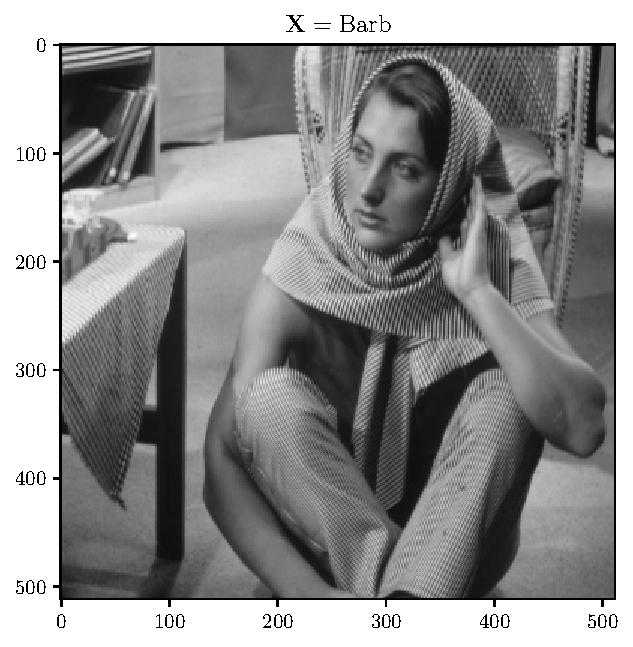
\includegraphics{barb}} & \href{https://nbviewer.org/github/vicente-gonzalez-ruiz/denoising/blob/main/figs/averaging_denoising.ipynb\#0MMGN_barb}{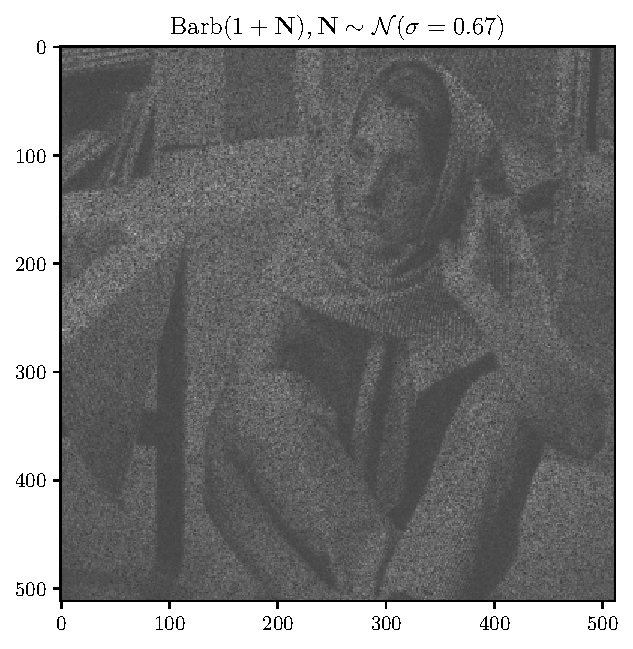
\includegraphics{0MMGN_barb}} \\
        \href{https://nbviewer.org/github/vicente-gonzalez-ruiz/denoising/blob/main/figs/averaging_denoising.ipynb\#denoised_0MMGN_barb}{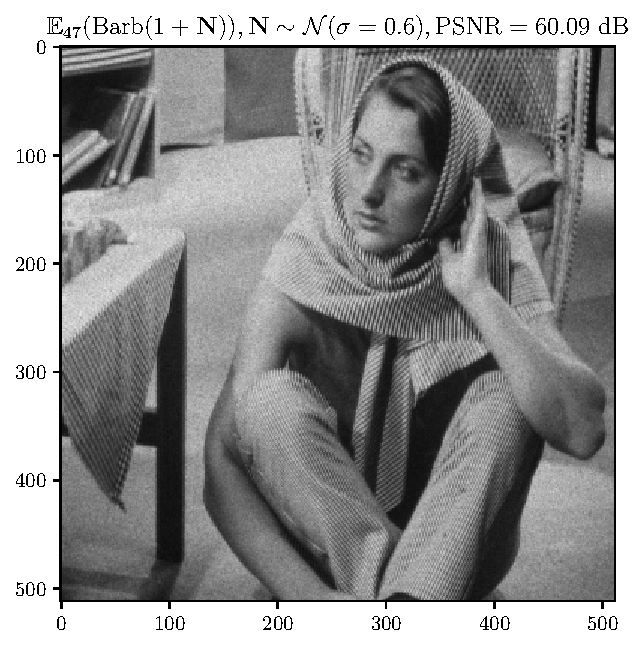
\includegraphics{denoised_0MMGN_barb}} & \href{https://nbviewer.org/github/vicente-gonzalez-ruiz/denoising/blob/main/figs/averaging_denoising.ipynb\#PSNR_0MMGN_barb}{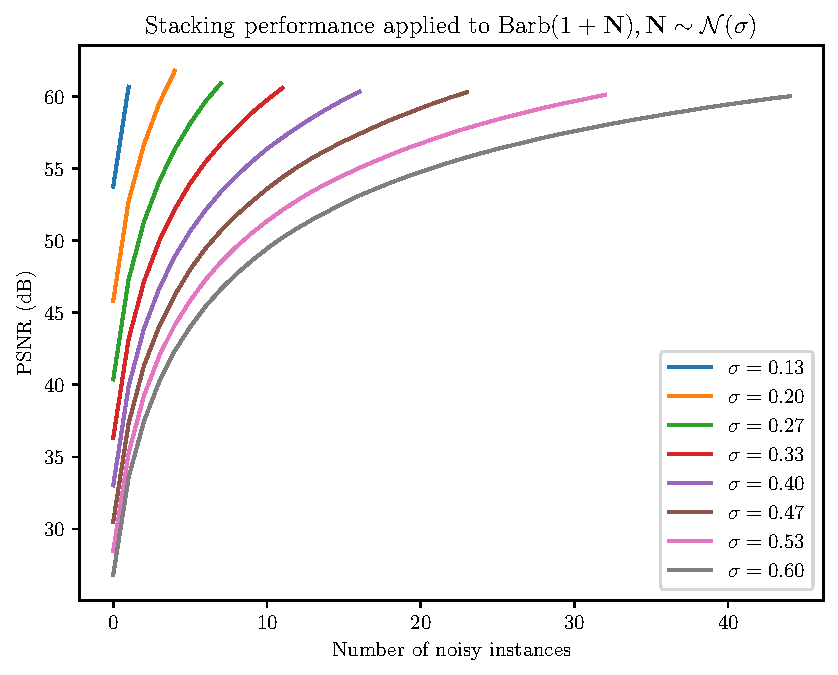
\includegraphics{PSNR_0MMGN_barb}}
      \end{tabular}
    }
    \caption{Effect of zero-mean multiplicative Gaussian noise in an
      image and how stacking can be used to reduced by stacking. The
      clean image of Barb is shown on the top left, and a noisy
      version on the top right. On to bottom, the left image shows a
      denoised version after stacking and the right graph shows the
      performance of the stacking process for different levels of
      noise.\label{fig:0MMGN}}
  \end{figure}
  
  Another distribution used for modeling speckle noise is the Rice
  distribution ($\mathbf{N}\sim\mathrm{Rice}(\nu,\sigma)$), with PDF
  \begin{equation}
    f(x; \nu,\sigma) = \Pr({\mathbf N}^{(i)}_j{=}x) = \frac{x}{\sigma^2}e^{\frac{-(x^2+\nu^2)}{2\sigma^2}}I_0\left(\frac{x\nu}{\sigma^2}\right),
  \end{equation}
  where $x$ is continuous, and $I_o$ is the modified Bessel function
  of the first kind with order zero. Rician noisy tensor instances can
  be generated with
  \begin{equation}
    \hat{\mathbf X}^{(i)} = \sqrt{ ({\mathbf X} + {\mathbf N}_{\text{real}}^{(i)})^2 + ({\mathbf N}_{\text{imag}}^{(i)})^2}.
  \end{equation}
  %Notice that the Rayleigh distribution ($\mathbf{N}\sim\mathrm{Rayleigh}(\sigma)$),
  %which is defined by the PDF
  %\begin{equation}
  %  {\mathbf N}^{(i)} \sim f(x; \sigma) = \frac{x}{\sigma^2} e^{-x^2/(2\sigma^2)}, \quad x \geq 0,
  %\end{equation}
  %continuous both, $x$ and $\sigma$ (the scale parameter) is a
  %particular case of Rice distribution when $\nu=0$.
  Notice that, even being $\nu=0$ (in whose case we are working with
  the Rayleigh distribution
  ($\mathbf{N}\sim\mathrm{Rayleigh}(\sigma)$)), the mean of the noise
  is not zero. The noise that corrupts magnetic resonance images is
  usually modeled as Rician/Rayleigh noise. Fig.~\ref{fig:Poisson}
  shows an example of how Rayleigh noise is cancelled by stacking.

  \begin{figure}
    \centering
    \resizebox{1.0\textwidth}{!}{
      \renewcommand{\arraystretch}{0.0} % Adjust row spacing in the table
      \setlength{\tabcolsep}{0ex}      % Adjust column spacing in the table    
      \begin{tabular}{cc}
        \href{https://nbviewer.org/github/vicente-gonzalez-ruiz/denoising/blob/main/figs/averaging_denoising.ipynb\#barb}{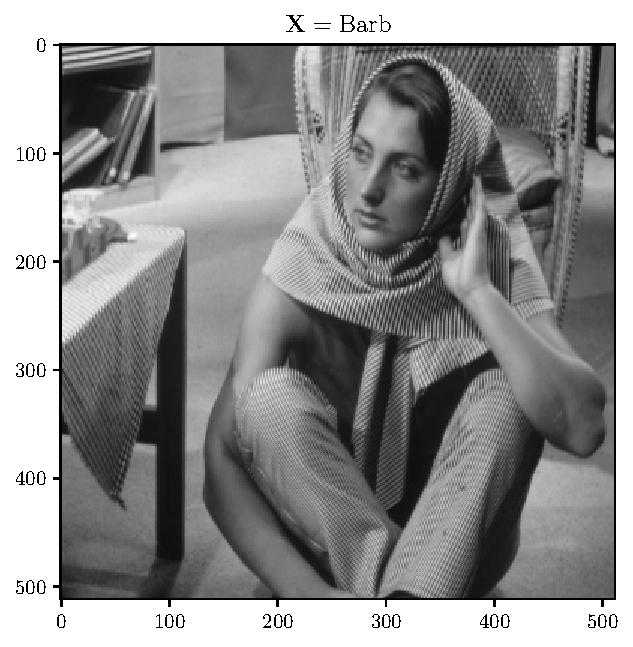
\includegraphics{barb}} & \href{https://nbviewer.org/github/vicente-gonzalez-ruiz/denoising/blob/main/figs/averaging_denoising.ipynb\#Rayleigh_barb}{\includegraphics{Rayleigh_barb}} \\
        \href{https://nbviewer.org/github/vicente-gonzalez-ruiz/denoising/blob/main/figs/averaging_denoising.ipynb\#denoised_Rayleigh_barb}{\includegraphics{denoised_Rayleigh_barb}} & \href{https://nbviewer.org/github/vicente-gonzalez-ruiz/denoising/blob/main/figs/averaging_denoising.ipynb\#PSNR_Rayleigh_barb}{\includegraphics{PSNR_Rayleigh_barb}}
      \end{tabular}
    }
    \caption{Effect of Rayleigh noise in an image and how stacking can
      be used to reduced by stacking. The clean image of Barb is shown
      on the top left, and a noisy version on the top right. On to
      bottom, the left image shows a denoised version after stacking
      and the right graph shows the performance of the stacking
      process for different levels of noise.\label{fig:Rayleigh}}
  \end{figure}

\item \textbf{Shot noise} modeled as Poisson noise
  ($\mathbf{N}\sim\mathrm{Poisson}(\lambda)$), with PMD (Probability Mass
  Distribution)\footnote{Also called discrete PDF.} equal to
  \begin{equation}
    f(k; \lambda={\mathbf X}) = \Pr({\mathbf N}^{(i)}{=}k) = \frac{\lambda^k e^{-\lambda}}{k!},
    \label{eq:PN}
  \end{equation}
  where both $f\in\mathbb{R}$, $k\in\mathbb{Z}$ are discrete ($f$
  describes the probability of $k$ events occurring within an observed
  interval (for example, of time) when, in average, we have
  $\lambda\in\mathbb{R}$ events in such interval size). Poisson noise
  can be significative in capturing devices that work with low doses
  of electrons, such as often happens in electron microscopy.
  Fig.~\ref{fig:Poisson} shows an example of how Poisson noise is
  cancelled by stacking.

  \begin{figure}
    \centering
    \resizebox{1.0\textwidth}{!}{
      \renewcommand{\arraystretch}{0.0} % Adjust row spacing in the table
      \setlength{\tabcolsep}{0ex}      % Adjust column spacing in the table    
      \begin{tabular}{cc}
        \href{https://nbviewer.org/github/vicente-gonzalez-ruiz/denoising/blob/main/figs/averaging_denoising.ipynb\#barb}{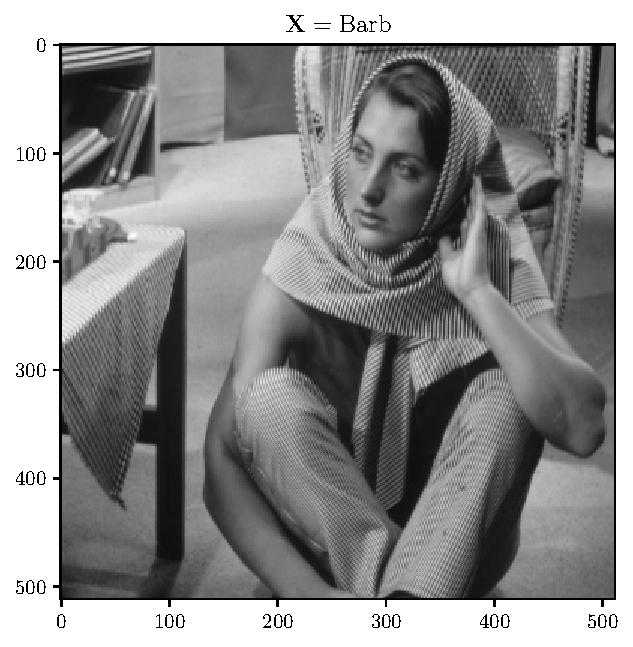
\includegraphics{barb}} & \href{https://nbviewer.org/github/vicente-gonzalez-ruiz/denoising/blob/main/figs/averaging_denoising.ipynb\#Poisson_barb}{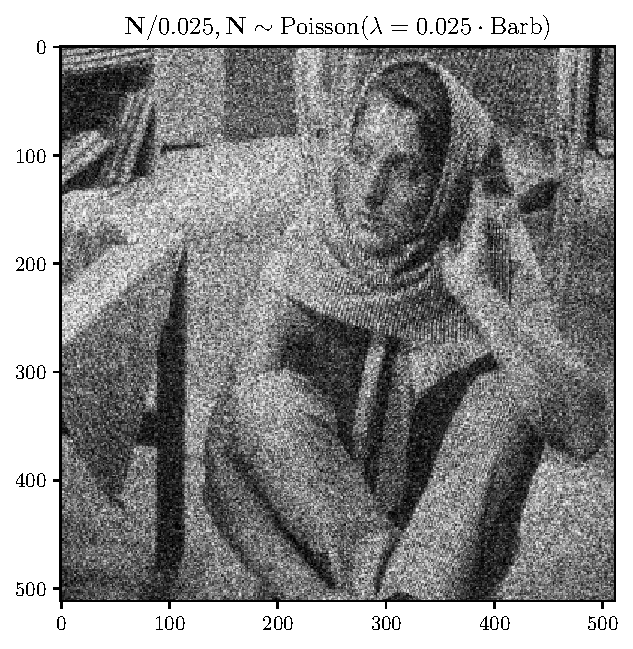
\includegraphics{Poisson_barb}} \\
        \href{https://nbviewer.org/github/vicente-gonzalez-ruiz/denoising/blob/main/figs/averaging_denoising.ipynb\#denoised_Poisson_barb}{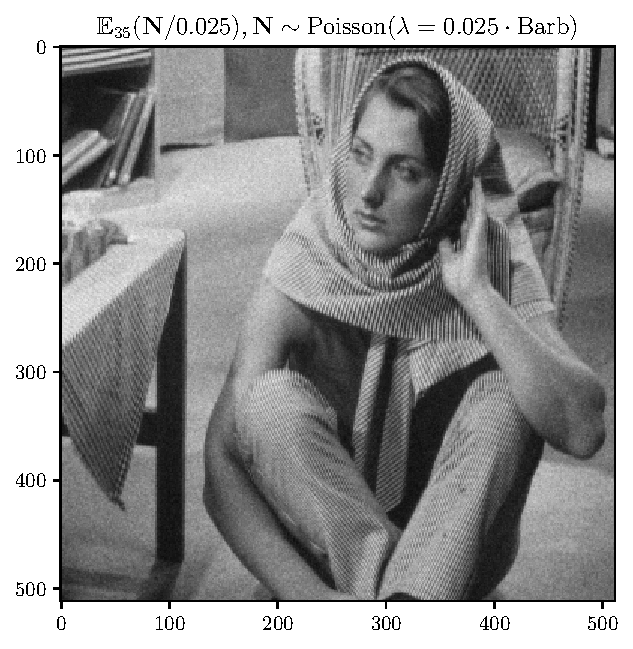
\includegraphics{denoised_Poisson_barb}} & \href{https://nbviewer.org/github/vicente-gonzalez-ruiz/denoising/blob/main/figs/averaging_denoising.ipynb\#PSNR_Poisson_barb}{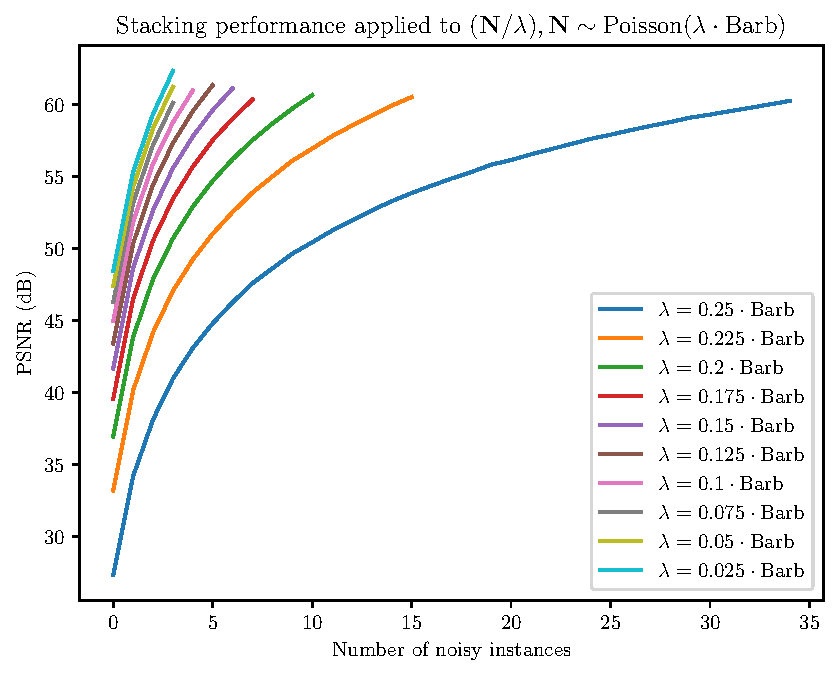
\includegraphics{PSNR_Poisson_barb}}
      \end{tabular}
    }
    \caption{Effect of Poisson noise in an image and how stacking can
      be used to reduced by stacking. The clean image of Barb is shown
      on the top left, and a noisy version on the top right. On to
      bottom, the left image shows a denoised version after stacking
      and the right graph shows the performance of the stacking
      process for different levels of noise.\label{fig:Poisson}}
  \end{figure}

\end{enumerate}

\section{Denoising techniques}

We consider denoising techniques where there is only one noisy
instance or a few instances, usually in the latter case with slightly
different versions of the clean signal. Stacking as such is therefore
excluded.

\subsection{Gaussian Denoising (GD)}

GD, also known by Gaussian smoothing filtering, works weight-averaging
signal samples. Under the assumption that most of the energy (and
information) is concentrated in the low frequencies, a Gaussian filter
(or kernel) is a low-pass filter defined by
\begin{equation}
  \mathbf{h}(\sigma) = \{\mathbf{h}_i(\sigma)\} = \frac{1}{\sqrt{2\pi}\sigma}e^{{-i}^2/(2\sigma^2)},
  \label{eq:GK}
\end{equation}
where $\sigma$ determines the cut-off frequency of the filter (a higher $\sigma$
results in a lower the cut-off frequency of the filter, and therefore,
in a higher smoothing effect).

1-D Gaussian filtering is represented by
\begin{equation}
  \hat{\mathbf{Y}}(\sigma) = \mathbf{Y}*\mathbf{h}(\sigma),
  \label{eq:GF}
\end{equation}
where $*$ represent the convolution of digital (in this case, 1D) signals.

As can be seen in Eq.~\ref{eq:GK} (all the kernel coefficients are
positive), GD requires only a noisy instance, and computes weighted
averages of neighbour signal samples. This does not mach the calculus
described in Eq.~\ref{eq:averaging_result}, but as an advantage, GD
requires only a noisy instance. The results is a smooth denoised
signal $\tilde{\mathbf X}$, but as we will see, this is a common
effect in all the denoising algorithms that work only with one noisy
instance.

Multidimensional Gaussian filters are separable, which means that we
can apply the 1D filter to all the dimensions of the signal to compute
a $N$D denoising. For the 3D case,
\begin{equation}
  \hat{\mathbf{Y}}(\sigma) = \Big(\big({\mathbf Y}*^{(\text{Z})}{\mathbf h}(\sigma)\big)*^{(\text{Y})}{\mathbf h}(\sigma)\Big)*^{(\text{X})}{\mathbf h}(\sigma),
    \label{eq:3DGF}
\end{equation}
where ${\mathbf s}*^{(d)}{\mathbf h}$ is the 1D convolution applied to
the dimension $d$ of the signal ${\mathbf s}$ and the 1D filter
${\mathbf h}$. For simplicity, Eq.~\ref{eq:3DGF} defines isotropic
filtering, but variance can be different at each dimension to provide
anisotropic filtering.

\section{SDPG (Structure-Preserving Gaussian Denoising) \cite{gonzalez2023structure}}

SDPG is based in 3D Gaussian filtering (Eq.~\ref{eq:3DGF}), but the noised
volume ${\mathbf Y}$ is dynamically warped to decrease the bluring at the
structures detected by an 2-D OF (Optical Flow) estimator:
\begin{equation}
  \hat{\mathbf{Y}}(\sigma; w, l) = \Big(\big(R_\text{Z}(\mathbf{Y}; w, l)*^{(\text{Z})}{\mathbf h}(\sigma)\big)*^{(\text{Y})}{\mathbf h}(\sigma)\Big)*^{(\text{X})}{\mathbf h}(\sigma),
    \label{eq:SDPG}
\end{equation}
where
\begin{equation*}
    \begin{array}{rclll}
    R_\text{Z}(\mathbf{Y}; w, l) & = & \big\{ \{ \overset{z'\rightarrow z}{\mathbf d}({\mathbf Y}_{[z',:,:]}; w, l)~:~\overset{z'\rightarrow z}{\mathbf d}({\mathbf Y}_{[z',:,:]})\approx{\mathbf Y}_{[z,:,:]} & \\ & & \text{for}
 ~z'=z-k,\cdots,z+k\} ~\text{for}~z=0,1,\cdots,N_\text{Z}-1\big\}, \\
    R_\text{Y}(\mathbf{Y}; w, l) & = & \big\{ \{ \overset{y'\rightarrow y}{\mathbf d}({\mathbf Y}_{[:,y',:]}; w, l)~:~\overset{y'\rightarrow y}{\mathbf d}({\mathbf Y}_{[:,y',:]}; w, l)\approx{\mathbf Y}_{[:,y,:]} & \\ & & \text{for}
 ~y'=y-k,\cdots,y+k\} ~\text{for}~y=0,1,\cdots,N_\text{Y}-1\big\},~\text{and} \\
    R_\text{X}(\mathbf{Y}; w, l) & = & \big\{ \{ \overset{x'\rightarrow x}{\mathbf d}({\mathbf Y}_{[:,:,x']}; w, l)~:~\overset{x'\rightarrow x}{\mathbf d}({\mathbf Y}_{[:,:,x']}; w, l)\approx{\mathbf Y}_{[:,:,x]} & \\ & & \text{for}
 ~x'=x-k,\cdots,x+k\} ~\text{for}~x=0,1,\cdots,N_\text{X}-1\big\}
    \end{array}
\end{equation*}
are the warped volumes. For example,
$\overset{x'\rightarrow x}{\mathbf d}({\mathbf Y}_{[:,:,x']}; w, l)$
represents the projection of the slice at coordinate $x'$ fulfilling
that
$\overset{x'\rightarrow x}{\mathbf d}({\mathbf Y}_{[:,:,x']}; w,
l)\approx{\mathbf Y}_{[:,:,x]}$. Notice that, for each possible offset
in ${\mathbf Z}$, ${\mathbf Y}$, and ${\mathbf X}$, a different set of
warped 2-D slices must be computed.

As indicated in Eq.~\ref{eq:SDPG}, the estimator requires 2 new
parameters:
\begin{enumerate}
\item $w$, the size of a 2D window used to analyze the 2D slices. If
  $w$ is large, the estimator is less sensitive to the noise but also
  the small structures are ignored. Therefore, higher $w$ values
  increases blurring.
\item $l$, that controls the maximun displacements that the
  estimator can generate. Blurring increases with $l$.
\end{enumerate}


% \section{AND}

% \section{N2V}
% A. Krull, T.-O. Buchholz, and F. Jug, “Noise2void-learning denoising
% from single noisy images,” in Proceedings of the IEEE/CVF conference
% on computer vision and pattern recognition, 2019, pp. 2129–2137.



\section{Cryo-CARE \cite{buchholz2019cryo}}
CARE (Content-Aware image REstoration) methods leverage
available knowledge about the data at hand ought to yield superior
restoration results \cite{weigert2018content}. Concretely, Cryo-CARE
is an implementation of Noise2Noise (N2N) \cite{lehtinen2018noise2noise}.

N2N is a ``supervised'' learning method for denoising where the model
(a U-Net) is trained on pairs of noisy images. However, unlike
clasical supervised denoising deep-learning based models, that
implement
\begin{equation}
  \underset{\theta}{\operatorname{arg\,min}} \, \sum_j L \big(f_\theta(\hat{\mathbf X}_j^{(1)}), {\mathbf X}_j\big)
\end{equation}
where $\{(\hat{\mathbf X}_j^{(1)}, {\mathbf X}_j)\}_{j=1}^M$ is the training
dataset, and $L$ is a given lost function such as the MSE (here higher
values mean worst results), N2N solves
\begin{equation}
  \underset{\theta}{\operatorname{arg\,min}} \, \sum_j L \big(f_\theta(\hat{\mathbf X}_j^{(1)}), {\mathbf X}_j^{(2)}\big).
\end{equation}
In other words, given two noisy versions
$\{\hat{\mathbf Y}^{(1)}, \hat{\mathbf Y}^{(2)}\}$ of the same (clean)
volume ${\mathbf Y}$, N2N learns to infeer a denoised volume
\begin{equation}
  \tilde{\mathbf Y}=\frac{1}{2}\big(f_\theta(\hat{\mathbf Y}^{(1)})+f_\theta(\hat{\mathbf Y}^{(2)})\big)\approx{\mathbf Y}.
\end{equation}
Obviously, better approximations to ${\mathbf Y}$ will be obtained
having more noisy instances, after averaing all the denoised volumes.

\section{NLM (Non Local Means)} 

\section{BM4D}

\section{2D-RSVD (2D Random Shuffing Volume Denoising}

\section{3D-RSVD (3D Random Shuffling Volume Denoising}


\bibliographystyle{plain}
\bibliography{signal_processing,microscopy,denoising}

\end{document}
